\documentclass[11pt,letterpaper]{article}
\PassOptionsToPackage{hyphens}{url}
\usepackage[margin=.83in,top=.8in,bottom=.8in,headheight=15pt]{geometry}
\usepackage[T1]{fontenc}
\usepackage{lmodern,amsmath,amssymb,mathtools,bm,booktabs,array,graphicx,tikz}
\usetikzlibrary{arrows.meta,positioning,calc,decorations.pathreplacing,patterns}
\definecolor{ink}{HTML}{17344D}\definecolor{accent}{HTML}{087E8B}\definecolor{pale}{HTML}{EDF5F5}\definecolor{gold}{HTML}{AD6B19}
\providecommand{\dd}{\,\mathrm{d}}\providecommand{\R}{\mathbb{R}}
\providecommand{\E}{\mathbb{E}}\providecommand{\Var}{\operatorname{Var}}
\providecommand{\Cov}{\operatorname{Cov}}\providecommand{\diag}{\operatorname{diag}}
\providecommand{\norm}[1]{\left\lVert#1\right\rVert}
\providecommand{\abs}[1]{\left|#1\right|}
\usepackage{microtype,hyperref,fancyhdr,enumitem,amsthm,sectsty,needspace}
\allsectionsfont{\raggedright}
\hypersetup{colorlinks=true,linkcolor=ink,urlcolor=accent,pdfauthor={Zan Ahmad},pdftitle={Embeddings and scaled dot-product attention / Lecture notes}}
\setlength{\parindent}{0pt}\setlength{\parskip}{6pt}\linespread{1.07}
\setlist{itemsep=3pt,topsep=4pt,leftmargin=*}
\emergencystretch=2em\clubpenalty=10000\widowpenalty=10000
\pagestyle{fancy}\fancyhf{}\fancyhead[L]{\small Scientific Computing in Python / 2027}\fancyhead[R]{\small Lecture 6}
\fancyfoot[L]{\footnotesize Zan Ahmad}\fancyfoot[R]{\footnotesize\thepage}\renewcommand{\headrulewidth}{.3pt}
\newtheorem{proposition}{Proposition}\newtheorem{theorem}{Theorem}\newtheorem{lemma}{Lemma}
\theoremstyle{definition}\newtheorem{definition}{Definition}\newtheorem{example}{Example}
\numberwithin{equation}{section}
\begin{document}
{\small\scshape Scientific Computing in Python / 2027\hfill Lecture 6}\par\medskip
{\raggedright\hyphenpenalty=10000\exhyphenpenalty=10000\LARGE\bfseries\color{ink} Embeddings and scaled dot-product attention\par}\medskip
{\small Lecture notes}\par\bigskip
Attention combines a set of value vectors using weights obtained from query-key comparisons. We shall calculate that operation explicitly, keep track of every matrix dimension, and derive its normalization and masking properties. The supplied example uses fixed invented coordinates. It illustrates the computation inside a larger learned system without treating the coordinates as semantic or scientific evidence.

\section{Embedding and projection matrices}
\hypertarget{note-embedding-and-projection-matrices}{}\label{note:embedding-and-projection-matrices}
{\small \href{slides.html\#frame=embedding-and-projection-matrices\&step=1}{Slides for this section}}\par
Let $X\in\R^{n\times d}$ contain one embedding row per position. Three linear maps produce queries, keys, and values. Queries and keys must have the same feature dimension for dot products; values may have a different dimension. The example's embeddings and matrices are hand-set, not learned from a corpus.

\[
Q=XW_Q\in\R^{n\times d_k},\quad
K=XW_K\in\R^{n\times d_k},\quad
V=XW_V\in\R^{n\times d_v}.
\]

The score matrix $QK^{\mathsf T}$ has shape $n\times n$.

\subsection*{Row and column meanings}
\[
S_{ij}=\frac{q_i^{\mathsf T}k_j}{\sqrt{d_k}}.
\]

Row $i$ fixes the query. Column $j$ identifies a key whose associated value may contribute to that query's output.
\section{Rowwise softmax}
\hypertarget{note-rowwise-softmax}{}\label{note:rowwise-softmax}
{\small \href{slides.html\#frame=rowwise-softmax\&step=1}{Slides for this section}}\par
For each query, exponentiate the scores and divide by their sum over allowed keys. The resulting weights are nonnegative and sum to one. Softmax weights describe this computational normalization; they are not automatically calibrated probabilities of a scientific claim.

\[
A_{ij}=\frac{e^{S_{ij}}}{\sum_{\ell}e^{S_{i\ell}}},\qquad
A_{ij}>0,\quad\sum_jA_{ij}=1.
\]

Normalization is performed independently for each row.

\subsection*{Stable normalization}
For any row constant $c$,
\[
\frac{e^{s_j-c}}{\sum_\ell e^{s_\ell-c}}
=\frac{e^{s_j}}{\sum_\ell e^{s_\ell}}.
\]

Choose $c=\max_j s_j$ to avoid exponentiating large positive numbers.
\section{Weighted values}
\hypertarget{note-weighted-values}{}\label{note:weighted-values}
{\small \href{slides.html\#frame=weighted-values\&step=1}{Slides for this section}}\par
The output row is the weighted sum of value rows. Since the weights are nonnegative and sum to one, it lies in their convex hull. At fixed queries, keys, and mask, the operation is linear in the values, although the whole attention map is nonlinear in its inputs because the weights also depend on them.

\[
Z=AV,\qquad z_i=\sum_j A_{ij}v_j.
\]

If every value is the same vector $v_*$, then $z_i=v_*$ for every row.

\subsection*{Scaling the values}
With $Q$, $K$ and the allowed-key set fixed,
\[
A(\alpha V+\beta W)=\alpha AV+\beta AW.
\]

Doubling $V$ doubles $Z$. Changing $Q$ generally changes the weights themselves.
\begin{center}\begin{minipage}{.98\linewidth}\centering
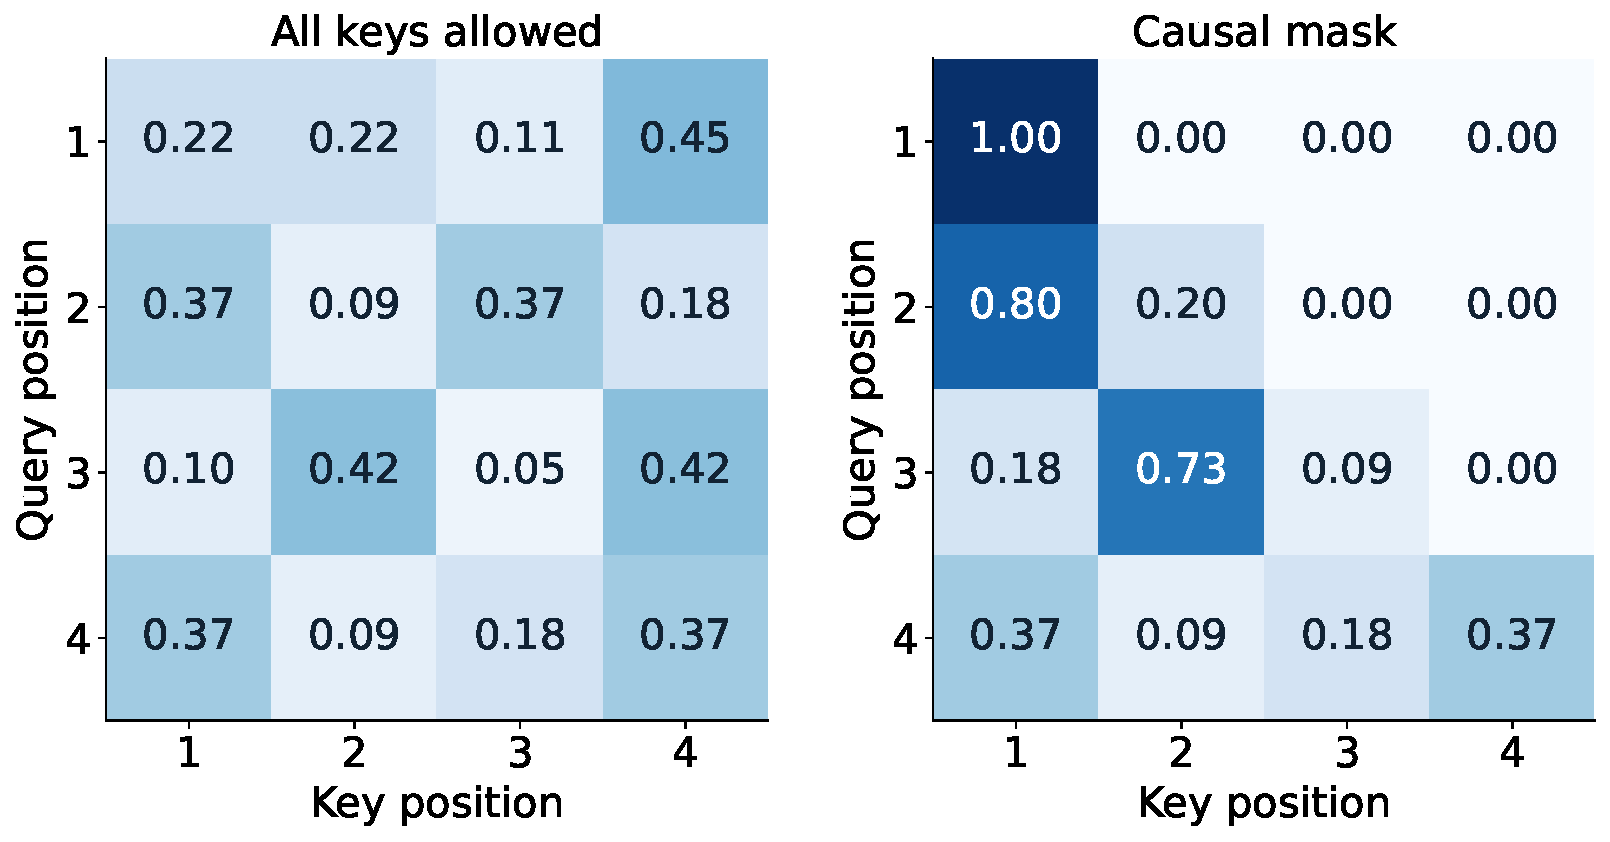
\includegraphics[width=.96\linewidth,height=.57\textheight,keepaspectratio]{attention-weights.pdf}\par\smallskip
{\small The same four hand-set embeddings and projections yield different row-normalized weights when future positions are disallowed. Decimal labels are rounded; tests use full precision.}
\end{minipage}\end{center}
\section{A two-key calculation}
\hypertarget{note-a-two-key-calculation}{}\label{note:a-two-key-calculation}
{\small \href{slides.html\#frame=a-two-key-calculation\&step=1}{Slides for this section}}\par
Take a query $(1,0)$ and keys $(1,0)$ and $(0,1)$, with $d_k=2$. The scores are $1/\sqrt2$ and zero. Pair the keys with values $(2,0)$ and $(0,4)$. The output illustrates how a scalar score weight multiplies an entire value vector.

\[
s=(1/\sqrt2,0),\qquad
A=\left(\frac{e^{1/\sqrt2}}{e^{1/\sqrt2}+1},\frac1{e^{1/\sqrt2}+1}\right).
\]

\[
A\approx(0.66976,0.33024).
\]

\subsection*{The output vector}
\[
z=0.66976(2,0)+0.33024(0,4)
\approx(1.33952,1.32096).
\]

The two output coordinates are value coordinates. They need not sum to one and are not token probabilities.
\section{Causal masking}
\hypertarget{note-causal-masking}{}\label{note:causal-masking}
{\small \href{slides.html\#frame=causal-masking\&step=1}{Slides for this section}}\par
A causal mask allows position $i$ to use keys only at positions $j\leq i$. Masked scores are excluded before normalization. Every row must retain at least one allowed key; an entirely masked row has no defined normalization. In a single attention layer with rowwise projections, changing a future embedding cannot alter earlier causal outputs.

\[
A_{ij}=0\quad(j>i),\qquad
\sum_{j\leq i}A_{ij}=1.
\]

The first position has only one allowed key, hence $A_{11}=1$.

\subsection*{A causal perturbation test}
Change only the final embedding row while holding projection matrices fixed.

Earlier causal outputs remain unchanged. Earlier unmasked outputs can change because the final key and value are available to them.
\begin{center}\begin{minipage}{.98\linewidth}\centering
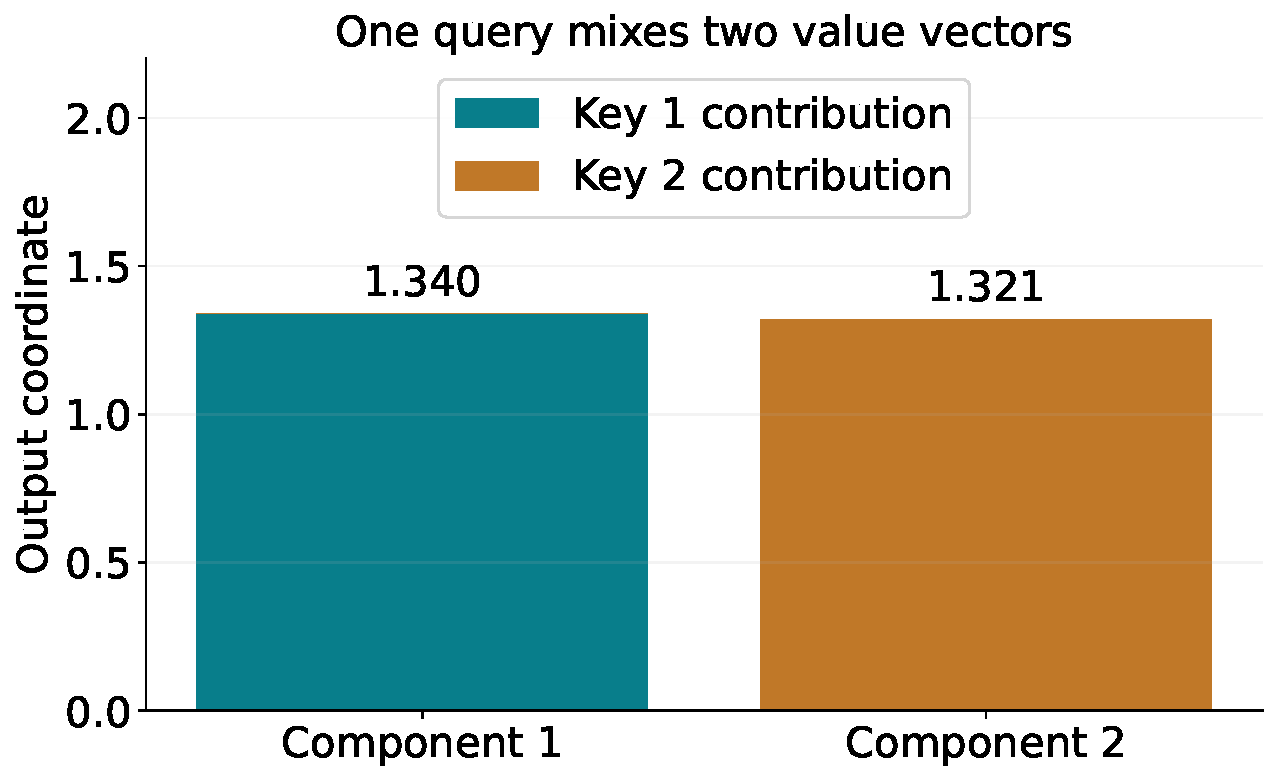
\includegraphics[width=.96\linewidth,height=.57\textheight,keepaspectratio]{weighted-values.pdf}\par\smallskip
{\small For the worked query and two keys, weighted contributions sum to [1.33952, 1.32095]. These invented output coordinates are not token probabilities or truth scores.}
\end{minipage}\end{center}
\section{Scaling and learned representations}
\hypertarget{note-scaling-and-learned-representations}{}\label{note:scaling-and-learned-representations}
{\small \href{slides.html\#frame=scaling-and-learned-representations\&step=1}{Slides for this section}}\par
If independent query and key coordinates have mean zero and variance one, their dot product has variance $d_k$. Division by $\sqrt{d_k}$ then gives a score with variance of order one. This motivates the scale under those assumptions. A transformer combines attention with additional operations and learns its parameters from a training objective; the fixed example establishes none of that learned behavior.

Under independent unit-variance coordinates,
\[
\operatorname{Var}\left(\sum_{r=1}^{d_k}q_rk_r\right)=d_k.
\]

Dividing by $\sqrt{d_k}$ keeps the variance at one.

\subsection*{Permutation and position}
Without positional information, permuting input rows by $P$ gives
\[
Q'=PQ,\ K'=PK,\ V'=PV\quad\Longrightarrow\quad Z'=PZ
\]
for unmasked attention.

Position encodings or structured masks provide information not present in an unordered collection of embedding rows.
\bigskip
\section*{Exercises}
\par\noindent\begin{minipage}{\linewidth}
\subsection*{P27-06-E1. Trace a new set of shapes}
There are 5 token positions, embedding width 4, query/key width 3 and value width 2.

\textbf{a} Give the shapes of X, WQ, WK and WV.

\end{minipage}\par\medskip
\textbf{b} Give the shapes of Q, K, V, the score table and Z.

\textbf{c} A proposed implementation multiplies Q@K instead of Q@K.T. Explain the error.

\par\noindent\begin{minipage}{\linewidth}
\subsection*{P27-06-E2. A transparent three-value mixture}
One query has equal scaled scores for three keys. Value rows are [3,0], [0,6] and [3,3].

\textbf{a} Find the normalized weights and output.

\end{minipage}\par\medskip
\textbf{b} Now allow only keys 1 and 3. Find the new weights and output.

\textbf{c} Why is zeroing the second old weight without renormalizing wrong?

\par\noindent\begin{minipage}{\linewidth}
\subsection*{P27-06-E3. Test information access}
A four-position self-attention calculation uses fixed projection matrices and a lower-triangular causal mask.

\textbf{a} Which output rows can change if only the embedding at position 4 changes?

\end{minipage}\par\medskip
\textbf{b} Does the same guarantee hold with all keys allowed?

\textbf{c} Specify a meaningful automated test and its limit.

\par\noindent\begin{minipage}{\linewidth}
\subsection*{P27-06-E4. Audit two automated claims}
A hypothetical explanation says: A, doubling all value coordinates doubles the output at fixed Q, K and mask; B, the largest weight proves which biological process caused an observation.

\textbf{a} Assess claim A algebraically.

\end{minipage}\par\medskip
\textbf{b} Assess claim B from the supplied demonstration.

\textbf{c} Give one code check for A and one evidence requirement for investigating B.

\section*{References}
\noindent\begin{minipage}{\linewidth}
Original Python Lecture 3. PDF pages 4--7, matrix prerequisites.

\end{minipage}\par\medskip
\noindent\begin{minipage}{\linewidth}
Vaswani and colleagues, Attention Is All You Need. Sections 3.2.1--3.2.3, equation 1; sections 3.4--3.5 for architecture context.

\url{https://arxiv.org/html/1706.03762v7}
\end{minipage}\par\medskip
Python source materials: Phillip Kerger (2023). Course adaptation and additional exposition: Zan Ahmad.

\end{document}
